\documentclass{standalone}
\usepackage[utf8]{inputenc}
\usepackage{pgfplots}
\DeclareUnicodeCharacter{2212}{−}
\usepgfplotslibrary{groupplots}
\usepgfplotslibrary{dateplot}
\usetikzlibrary{patterns}
\usetikzlibrary{shapes.arrows}
\pgfplotsset{compat=newest}
\begin{document}
% This file was created by tikzplotlib v0.9.1.
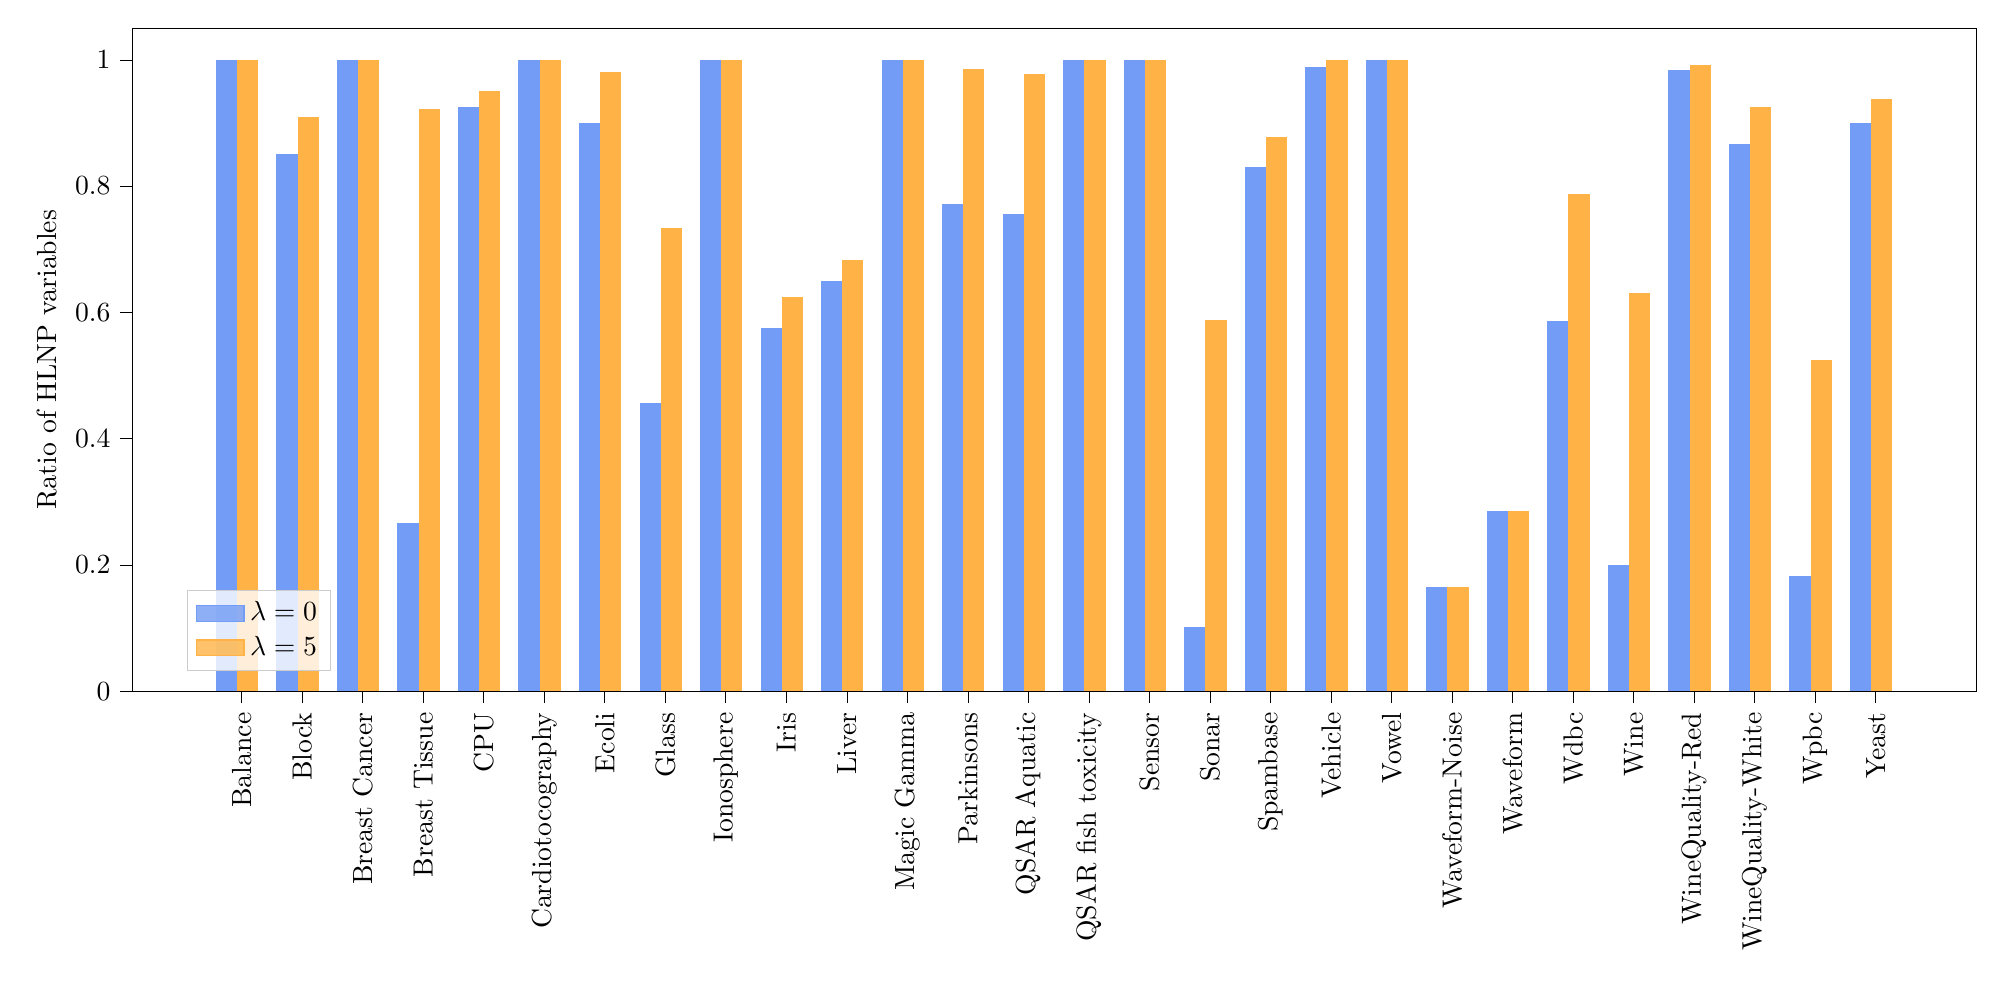
\begin{tikzpicture}

\definecolor{color0}{rgb}{0.447058823529412,0.611764705882353,0.96078431372549}
\definecolor{color1}{rgb}{1,0.701960784313725,0.274509803921569}

\begin{axis}[
height=10cm,
legend cell align={left},
legend style={fill opacity=0.8, draw opacity=1, text opacity=1, draw=white!80!black},
tick align=outside,
tick pos=left,
width=25cm,
x grid style={white!69.0196078431373!black},
xmin=-1.56, xmax=28.91,
xtick style={color=black},
xtick={0.25,1.25,2.25,3.25,4.25,5.25,6.25,7.25,8.25,9.25,10.25,11.25,12.25,13.25,14.25,15.25,16.25,17.25,18.25,19.25,20.25,21.25,22.25,23.25,24.25,25.25,26.25,27.25},
xticklabel style = {rotate=90.0},
xticklabels={Balance,Block,Breast Cancer,Breast Tissue,CPU,Cardiotocography,Ecoli,Glass,Ionosphere,Iris,Liver,Magic Gamma,Parkinsons,QSAR Aquatic,QSAR fish toxicity,Sensor,Sonar,Spambase,Vehicle,Vowel,Waveform-Noise,Waveform,Wdbc,Wine,WineQuality-Red,WineQuality-White,Wpbc,Yeast},
y grid style={white!69.0196078431373!black},
ylabel={Ratio of HLNP variables},
ymin=0, ymax=1.05,
ytick style={color=black},
legend pos = south west
]
\draw[draw=none,fill=color0] (axis cs:-0.175,0) rectangle (axis cs:0.175,1);
\draw[draw=none,fill=color0] (axis cs:0.825,0) rectangle (axis cs:1.175,0.85);
\draw[draw=none,fill=color0] (axis cs:1.825,0) rectangle (axis cs:2.175,1);
\draw[draw=none,fill=color0] (axis cs:2.825,0) rectangle (axis cs:3.175,0.266666666666667);
\draw[draw=none,fill=color0] (axis cs:3.825,0) rectangle (axis cs:4.175,0.925);
\draw[draw=none,fill=color0] (axis cs:4.825,0) rectangle (axis cs:5.175,1);
\draw[draw=none,fill=color0] (axis cs:5.825,0) rectangle (axis cs:6.175,0.9);
\draw[draw=none,fill=color0] (axis cs:6.825,0) rectangle (axis cs:7.175,0.455555555555555);
\draw[draw=none,fill=color0] (axis cs:7.825,0) rectangle (axis cs:8.175,1);
\draw[draw=none,fill=color0] (axis cs:8.825,0) rectangle (axis cs:9.175,0.575);
\draw[draw=none,fill=color0] (axis cs:9.825,0) rectangle (axis cs:10.175,0.65);
\draw[draw=none,fill=color0] (axis cs:10.825,0) rectangle (axis cs:11.175,1);
\draw[draw=none,fill=color0] (axis cs:11.825,0) rectangle (axis cs:12.175,0.771428571428571);
\draw[draw=none,fill=color0] (axis cs:12.825,0) rectangle (axis cs:13.175,0.755555555555556);
\draw[draw=none,fill=color0] (axis cs:13.825,0) rectangle (axis cs:14.175,1);
\draw[draw=none,fill=color0] (axis cs:14.825,0) rectangle (axis cs:15.175,1);
\draw[draw=none,fill=color0] (axis cs:15.825,0) rectangle (axis cs:16.175,0.101666666666667);
\draw[draw=none,fill=color0] (axis cs:16.825,0) rectangle (axis cs:17.175,0.829824561403509);
\draw[draw=none,fill=color0] (axis cs:17.825,0) rectangle (axis cs:18.175,0.988888888888889);
\draw[draw=none,fill=color0] (axis cs:18.825,0) rectangle (axis cs:19.175,1);
\draw[draw=none,fill=color0] (axis cs:19.825,0) rectangle (axis cs:20.175,0.165);
\draw[draw=none,fill=color0] (axis cs:20.825,0) rectangle (axis cs:21.175,0.285714285714286);
\draw[draw=none,fill=color0] (axis cs:21.825,0) rectangle (axis cs:22.175,0.586666666666667);
\draw[draw=none,fill=color0] (axis cs:22.825,0) rectangle (axis cs:23.175,0.2);
\draw[draw=none,fill=color0] (axis cs:23.825,0) rectangle (axis cs:24.175,0.983333333333333);
\draw[draw=none,fill=color0] (axis cs:24.825,0) rectangle (axis cs:25.175,0.866666666666667);
\draw[draw=none,fill=color0] (axis cs:25.825,0) rectangle (axis cs:26.175,0.181818181818182);
\draw[draw=none,fill=color0] (axis cs:26.825,0) rectangle (axis cs:27.175,0.9);
\draw[draw=none,fill=color1] (axis cs:0.175,0) rectangle (axis cs:0.525,1);
\draw[draw=none,fill=color1] (axis cs:1.175,0) rectangle (axis cs:1.525,0.91);
\draw[draw=none,fill=color1] (axis cs:2.175,0) rectangle (axis cs:2.525,1);
\draw[draw=none,fill=color1] (axis cs:3.175,0) rectangle (axis cs:3.525,0.922222222222222);
\draw[draw=none,fill=color1] (axis cs:4.175,0) rectangle (axis cs:4.525,0.95);
\draw[draw=none,fill=color1] (axis cs:5.175,0) rectangle (axis cs:5.525,1);
\draw[draw=none,fill=color1] (axis cs:6.175,0) rectangle (axis cs:6.525,0.98);
\draw[draw=none,fill=color1] (axis cs:7.175,0) rectangle (axis cs:7.525,0.733333333333333);
\draw[draw=none,fill=color1] (axis cs:8.175,0) rectangle (axis cs:8.525,1);
\draw[draw=none,fill=color1] (axis cs:9.175,0) rectangle (axis cs:9.525,0.625);
\draw[draw=none,fill=color1] (axis cs:10.175,0) rectangle (axis cs:10.525,0.683333333333333);
\draw[draw=none,fill=color1] (axis cs:11.175,0) rectangle (axis cs:11.525,1);
\draw[draw=none,fill=color1] (axis cs:12.175,0) rectangle (axis cs:12.525,0.985714285714286);
\draw[draw=none,fill=color1] (axis cs:13.175,0) rectangle (axis cs:13.525,0.977777777777778);
\draw[draw=none,fill=color1] (axis cs:14.175,0) rectangle (axis cs:14.525,1);
\draw[draw=none,fill=color1] (axis cs:15.175,0) rectangle (axis cs:15.525,1);
\draw[draw=none,fill=color1] (axis cs:16.175,0) rectangle (axis cs:16.525,0.588333333333333);
\draw[draw=none,fill=color1] (axis cs:17.175,0) rectangle (axis cs:17.525,0.87719298245614);
\draw[draw=none,fill=color1] (axis cs:18.175,0) rectangle (axis cs:18.525,1);
\draw[draw=none,fill=color1] (axis cs:19.175,0) rectangle (axis cs:19.525,1);
\draw[draw=none,fill=color1] (axis cs:20.175,0) rectangle (axis cs:20.525,0.165);
\draw[draw=none,fill=color1] (axis cs:21.175,0) rectangle (axis cs:21.525,0.285714285714286);
\draw[draw=none,fill=color1] (axis cs:22.175,0) rectangle (axis cs:22.525,0.786666666666667);
\draw[draw=none,fill=color1] (axis cs:23.175,0) rectangle (axis cs:23.525,0.630769230769231);
\draw[draw=none,fill=color1] (axis cs:24.175,0) rectangle (axis cs:24.525,0.991666666666667);
\draw[draw=none,fill=color1] (axis cs:25.175,0) rectangle (axis cs:25.525,0.925);
\draw[draw=none,fill=color1] (axis cs:26.175,0) rectangle (axis cs:26.525,0.524242424242424);
\draw[draw=none,fill=color1] (axis cs:27.175,0) rectangle (axis cs:27.525,0.9375);

\addlegendimage{area legend,fill=color0, color=color0}
\addlegendimage{area legend,fill=color1, color=color1}
\legend{$\lambda = 0$, $\lambda = 5$}
\end{axis}

\end{tikzpicture}

\end{document}
